\documentclass[aspectratio=169,10pt]{beamer}

\usepackage[T1]{fontenc}
\usepackage{lmodern}
\usepackage{booktabs}
\usepackage{tabularx}
\usepackage{tikz}
\usetikzlibrary{arrows.meta,positioning,fit}

\definecolor{HopkinsBlue}{HTML}{002D72}
\definecolor{SpiritBlue}{HTML}{68ACE5}
\definecolor{DeepBlue}{HTML}{001B44}
\definecolor{PaleBlue}{HTML}{EAF4FB}
\definecolor{Muted}{HTML}{526777}
\definecolor{Success}{HTML}{287A57}
\definecolor{Attention}{HTML}{B65738}

\setbeamercolor{normal text}{fg=DeepBlue,bg=white}
\setbeamercolor{structure}{fg=HopkinsBlue}
\setbeamercolor{frametitle}{fg=white,bg=HopkinsBlue}
\setbeamercolor{title}{fg=HopkinsBlue}
\setbeamercolor{subtitle}{fg=Muted}
\setbeamercolor{block title}{fg=white,bg=HopkinsBlue}
\setbeamercolor{block body}{fg=DeepBlue,bg=PaleBlue}
\setbeamercolor{alerted text}{fg=Attention}
\setbeamertemplate{navigation symbols}{}
\setbeamertemplate{itemize item}{\color{SpiritBlue}$\blacktriangleright$}
\setbeamertemplate{itemize subitem}{\color{HopkinsBlue}$\bullet$}
\setbeamertemplate{footline}{%
  \leavevmode\hbox{%
    \begin{beamercolorbox}[wd=.82\paperwidth,ht=2.6ex,dp=1.1ex,leftskip=1em]{author in head/foot}%
      \color{Muted}\scriptsize Digital Professor --- Interaction and Integration Specification
    \end{beamercolorbox}%
    \begin{beamercolorbox}[wd=.18\paperwidth,ht=2.6ex,dp=1.1ex,rightskip=1em plus1fil]{date in head/foot}%
      \color{Muted}\scriptsize\hfill\insertframenumber/\inserttotalframenumber
    \end{beamercolorbox}}}
\setbeamertemplate{frametitle}{%
  \nointerlineskip
  \begin{beamercolorbox}[wd=\paperwidth,ht=3.15ex,dp=1.15ex,leftskip=.55cm]{frametitle}%
    \insertframetitle
  \end{beamercolorbox}}

\title{Interaction and Integration Specification}
\subtitle{What is defined, how the pieces connect, and what comes next}
\author{Jonathan Ma}
\institute{Digital Professor}
\date{October 2026}

\begin{document}

% Suggested time: 0:30
\begin{frame}[plain]
  \vfill
  {\usebeamerfont{title}\color{HopkinsBlue}\LARGE\inserttitle\par}
  \vspace{.5em}
  {\color{Muted}\large\insertsubtitle\par}
  \vspace{1.4em}
  {\color{SpiritBlue}\rule{2.4cm}{2pt}}\par
  \vspace{1.2em}
  {\small\insertauthor\hfill\insertdate}
  \vfill
\end{frame}

% Suggested time: 1:10
\begin{frame}{Why we moved into a specification phase}
\begin{block}{The integration problem}
We have working ideas for course ingestion, retrieval, multimodal interaction, tutoring decisions, and delivery. The next risk is that each part assumes different inputs, outputs, or ownership.
\end{block}
\vspace{.55em}
\begin{columns}[T,onlytextwidth]
\column{.31\textwidth}
\begin{block}{Define}
State what each component is responsible for and what it must not do.
\end{block}
\column{.31\textwidth}
\begin{block}{Connect}
Give every handoff a producer, consumer, record, status, and failure path.
\end{block}
\column{.34\textwidth}
\begin{block}{Review}
Resolve disagreements in Markdown before they become incompatible code.
\end{block}
\end{columns}
\vspace{.55em}
\centering
\textbf{Current goal:} create an implementable system contract, then build against it.
\end{frame}

% Suggested time: 1:30
\begin{frame}{The proposed tutoring loop}
\centering
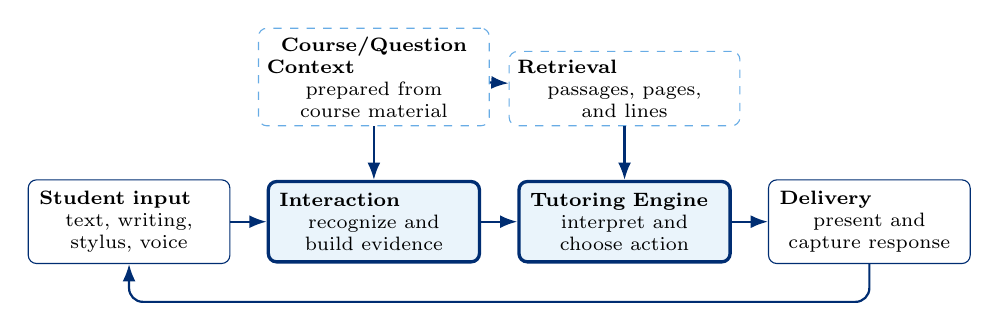
\begin{tikzpicture}[
  node distance=.52cm and .46cm,
  box/.style={draw=HopkinsBlue,rounded corners=3pt,fill=white,align=center,text width=2.28cm,minimum height=.95cm,inner sep=4pt,font=\scriptsize},
  focus/.style={draw=HopkinsBlue,very thick,rounded corners=3pt,fill=PaleBlue,align=center,text width=2.40cm,minimum height=1.02cm,inner sep=4pt,font=\scriptsize},
  support/.style={draw=SpiritBlue,dashed,rounded corners=3pt,fill=white,align=center,text width=2.72cm,minimum height=.80cm,inner sep=3pt,font=\scriptsize},
  arrow/.style={-{Latex[length=2.2mm]},thick,draw=HopkinsBlue}]

\node[box] (student) {\textbf{Student input}\newline text, writing, stylus, voice};
\node[focus,right=of student] (interaction) {\textbf{Interaction}\newline recognize and build evidence};
\node[focus,right=of interaction] (engine) {\textbf{Tutoring Engine}\newline interpret and choose action};
\node[box,right=of engine] (delivery) {\textbf{Delivery}\newline present and capture response};
\node[support,above=.68cm of interaction] (context) {\textbf{Course/Question Context}\newline prepared from course material};
\node[support,above=.68cm of engine] (retrieval) {\textbf{Retrieval}\newline passages, pages, and lines};

\draw[arrow] (student)--(interaction);
\draw[arrow] (interaction)--(engine);
\draw[arrow] (engine)--(delivery);
\draw[arrow] (context)--(interaction);
\draw[arrow] (context)--(retrieval);
\draw[arrow] (retrieval)--(engine);
\draw[arrow,rounded corners=5pt] (delivery.south) -- ++(0,-.48) -| (student.south);
\end{tikzpicture}
\vspace{.55em}

\small
Each response becomes new evidence. The system reassesses and chooses the next action instead of treating messages as isolated questions.
\end{frame}

% Suggested time: 1:20
\begin{frame}{My module: the interaction boundary}
\begin{columns}[T,onlytextwidth]
\column{.48\textwidth}
\begin{block}{What it owns}
\begin{itemize}
\item Capture and preserve student submissions
\item Route handwriting and voice recognition
\item Confirm meaning-changing ambiguity
\item Build factual Student Evidence
\item Link attempts, help, and revisions
\item Coordinate turn handoffs and status
\end{itemize}
\end{block}
\column{.49\textwidth}
\begin{block}{What stays downstream}
\begin{itemize}
\item Mathematical correctness judgments
\item Misconception or mastery diagnosis
\item Course-passage ranking
\item Selection of hints or explanations
\item Avatar and channel presentation
\end{itemize}
\end{block}
\end{columns}
\vspace{.45em}
\centering
\textbf{Boundary rule:} preserve what the student did; let the Tutoring Engine decide what it means.
\end{frame}

% Suggested time: 1:15
\begin{frame}{Practical V1 input scope}
\small
\begin{tabularx}{\textwidth}{@{}p{.24\textwidth}p{.18\textwidth}X@{}}
\toprule
\textbf{Input} & \textbf{V1} & \textbf{Approach} \\
\midrule
Typed text and TeX & Include & Baseline input with original source preserved separately from rendering. \\
\addlinespace
Handwritten image/PDF & Include & One visual-recognition path with confirmation for important ambiguity. \\
\addlinespace
Direct stylus input & Include & Export the canvas and reuse the handwriting path. \\
\addlinespace
Voice & Simplify & Record one audio clip, transcribe it, and allow confirmation or editing. \\
\addlinespace
Live voice/video/avatar & Defer & Add after the asynchronous tutoring loop and delivery contracts are stable. \\
\bottomrule
\end{tabularx}
\vspace{.55em}
\begin{block}{Why this scope}
It tests the evidence and handoff design across realistic modalities without requiring multiple real-time systems at once.
\end{block}
\end{frame}

% Suggested time: 1:40
\begin{frame}{From a submission to Student Evidence}
\centering
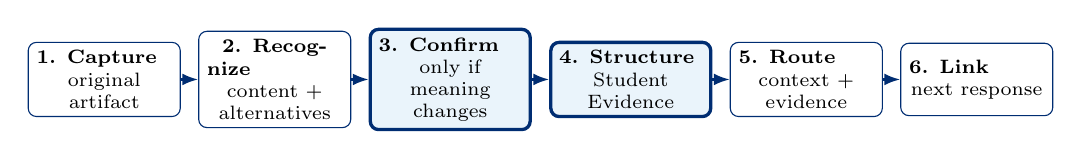
\begin{tikzpicture}[
  node distance=.22cm,
  box/.style={draw=HopkinsBlue,rounded corners=3pt,fill=white,align=center,text width=1.72cm,minimum height=.92cm,inner sep=3pt,font=\scriptsize},
  focus/.style={draw=HopkinsBlue,very thick,rounded corners=3pt,fill=PaleBlue,align=center,text width=1.82cm,minimum height=.92cm,inner sep=3pt,font=\scriptsize},
  arrow/.style={-{Latex[length=2mm]},thick,draw=HopkinsBlue}]
\node[box] (capture) {\textbf{1. Capture}\newline original artifact};
\node[box,right=of capture] (recognize) {\textbf{2. Recognize}\newline content + alternatives};
\node[focus,right=of recognize] (confirm) {\textbf{3. Confirm}\newline only if meaning changes};
\node[focus,right=of confirm] (evidence) {\textbf{4. Structure}\newline Student Evidence};
\node[box,right=of evidence] (route) {\textbf{5. Route}\newline context + evidence};
\node[box,right=of route] (link) {\textbf{6. Link}\newline next response};
\draw[arrow] (capture)--(recognize);
\draw[arrow] (recognize)--(confirm);
\draw[arrow] (confirm)--(evidence);
\draw[arrow] (evidence)--(route);
\draw[arrow] (route)--(link);
\end{tikzpicture}
\vspace{.75em}
\begin{columns}[T,onlytextwidth]
\column{.48\textwidth}
\begin{block}{Evidence records facts}
Original work, confirmed transcription, observable steps, final answer, explanation, stated uncertainty, prior help, and revision links.
\end{block}
\column{.49\textwidth}
\begin{block}{Learner State interprets facts}
What appears understood, what remains unresolved, and which gap or misconception is plausible.
\end{block}
\end{columns}
\end{frame}

% Suggested time: 1:25
\begin{frame}{Ambiguity: confirm meaning, not every character}
\begin{columns}[T,onlytextwidth]
\column{.47\textwidth}
\begin{block}{Example}
A handwritten expression could be read as:
\[
  x_1+x_2=1
\]
or
\[
  x_l+x_2=l
\]
\end{block}
\column{.50\textwidth}
\begin{block}{Expected behavior}
\begin{enumerate}
\item Preserve the original image
\item Store both recognition candidates
\item Show the relevant crop to the student
\item Ask for a selection or free-form edit
\item Log raw and corrected values separately
\item Mark unresolved evidence as unconfirmed
\end{enumerate}
\end{block}
\end{columns}
\vspace{.45em}
\centering
\alert{\textbf{The recognizer must not silently change an incorrect student equation into a correct one.}}
\end{frame}

% Suggested time: 1:35
\begin{frame}{The shared records connect the modules}
\small
\begin{tabularx}{\textwidth}{@{}>{\raggedright\arraybackslash}p{.22\textwidth}>{\raggedright\arraybackslash}p{.25\textwidth}>{\raggedright\arraybackslash}X@{}}
\toprule
\textbf{Record} & \textbf{Handoff} & \textbf{Purpose} \\
\midrule
\texttt{CourseContext} and \texttt{QuestionContext} & Ingestion $\rightarrow$ system & Identify the course, question, objectives, rules, and approved source versions. \\
\addlinespace
\texttt{StudentEvidence} & Interaction $\rightarrow$ Tutoring Engine & Preserve the student's confirmed work and its history. \\
\addlinespace
\texttt{RetrievalRequest} / \texttt{GroundingBundle} & System $\leftrightarrow$ Retrieval & Ask for and return relevant course passages. \\
\addlinespace
\texttt{LearnerState} / \texttt{TutoringAction} & Tutoring Engine $\rightarrow$ Delivery & Explain the current interpretation and prescribe one next action. \\
\addlinespace
\texttt{DeliveryResult} & Delivery $\rightarrow$ Interaction & Record what was actually presented and continue the turn. \\
\bottomrule
\end{tabularx}
\vspace{.45em}
\centering
The draft interface specification defines required IDs, status, provenance, validation, and failure behavior for each record.
\end{frame}

% Suggested time: 1:25
\begin{frame}{Grounding and logging are part of the contract}
\begin{columns}[T,onlytextwidth]
\column{.48\textwidth}
\begin{block}{Precise course grounding}
\begin{itemize}
\item Store a passage, page, and normalized line range
\item Retain document and content-version identifiers
\item Provide an authorized highlight link
\item Return \texttt{no\_support\_found} instead of inventing a citation
\end{itemize}
\end{block}
\column{.49\textwidth}
\begin{block}{Configurable logging}
\begin{itemize}
\item Separate required session state from diagnostics
\item Allow optional logging to be turned on or off
\item Keep raw and corrected recognition distinct
\item Record versions, status, latency, retries, and cost when available
\end{itemize}
\end{block}
\end{columns}
\vspace{.5em}
\centering
\textbf{Traceability target:} connect a tutoring action to the evidence, course passage, and component versions that produced it.
\end{frame}

% Suggested time: 1:15
\begin{frame}{What is complete in the first draft}
\begin{columns}[T,onlytextwidth]
\column{.49\textwidth}
\begin{block}{Shared specification}
\begin{itemize}
\item Repository structure and module template
\item High-level architecture and tutoring workflow
\item Initial shared-record definitions
\item Logging, correction, grounding, and failure rules
\end{itemize}
\end{block}
\column{.48\textwidth}
\begin{block}{Interaction specification}
\begin{itemize}
\item V1 modality recommendation
\item Recognition and ambiguity behavior
\item Student Evidence and revision links
\item Handoffs to context, retrieval, tutoring, and delivery
\item Acceptance scenarios and open questions
\end{itemize}
\end{block}
\end{columns}
\vspace{.55em}
\centering
\textbf{Status:} reviewable V0.1 contracts, not a frozen architecture or completed implementation.
\end{frame}

% Suggested time: 1:30
\begin{frame}{What teammates are reviewing now}
\begin{columns}[T,onlytextwidth]
\column{.31\textwidth}
\begin{block}{Ovunc}
Course and Question Context, ingestion behavior, source versions, normalized pages, and stable line mappings.
\end{block}
\column{.31\textwidth}
\begin{block}{Sean}
Retrieval requests, chunk/index versions, passage ranking, page/line citations, and highlight links.
\end{block}
\column{.34\textwidth}
\begin{block}{Yining}
Tutoring Action requirements, avatar/channel presentation, Delivery Result, and return of the next response.
\end{block}
\end{columns}
\vspace{.65em}
\begin{block}{The purpose of review}
Each teammate should change the shared interfaces when their module cannot reliably produce or consume what the current draft assumes.
\end{block}
\end{frame}

% Suggested time: 1:35
\begin{frame}{Next: resolve contracts, then implement one slice}
\begin{columns}[T,onlytextwidth]
\column{.48\textwidth}
\begin{block}{Decisions to resolve}
\begin{itemize}
\item Who creates the final retrieval request?
\item Which Question Context fields are guaranteed?
\item How do page/line mappings remain stable?
\item What evidence is sufficient for Learner State?
\item Where does recognition confirmation end and tutoring begin?
\end{itemize}
\end{block}
\column{.49\textwidth}
\begin{block}{Implementation sequence}
\begin{enumerate}
\item Reconcile teammate module specifications
\item Finalize Tutoring Engine and Delivery contracts
\item Freeze interface version 0.1
\item Implement one text-first tutoring loop
\item Add handwriting, stylus, and recorded voice paths
\item Validate with a Calculus scenario set and independent math review
\end{enumerate}
\end{block}
\end{columns}
\end{frame}

\end{document}
